\documentclass{article}\usepackage[]{graphicx}\usepackage[]{color}
%% maxwidth is the original width if it is less than linewidth
%% otherwise use linewidth (to make sure the graphics do not exceed the margin)
\makeatletter
\def\maxwidth{ %
  \ifdim\Gin@nat@width>\linewidth
    \linewidth
  \else
    \Gin@nat@width
  \fi
}
\makeatother

\definecolor{fgcolor}{rgb}{0.345, 0.345, 0.345}
\newcommand{\hlnum}[1]{\textcolor[rgb]{0.686,0.059,0.569}{#1}}%
\newcommand{\hlstr}[1]{\textcolor[rgb]{0.192,0.494,0.8}{#1}}%
\newcommand{\hlcom}[1]{\textcolor[rgb]{0.678,0.584,0.686}{\textit{#1}}}%
\newcommand{\hlopt}[1]{\textcolor[rgb]{0,0,0}{#1}}%
\newcommand{\hlstd}[1]{\textcolor[rgb]{0.345,0.345,0.345}{#1}}%
\newcommand{\hlkwa}[1]{\textcolor[rgb]{0.161,0.373,0.58}{\textbf{#1}}}%
\newcommand{\hlkwb}[1]{\textcolor[rgb]{0.69,0.353,0.396}{#1}}%
\newcommand{\hlkwc}[1]{\textcolor[rgb]{0.333,0.667,0.333}{#1}}%
\newcommand{\hlkwd}[1]{\textcolor[rgb]{0.737,0.353,0.396}{\textbf{#1}}}%
\let\hlipl\hlkwb

\usepackage{framed}
\makeatletter
\newenvironment{kframe}{%
 \def\at@end@of@kframe{}%
 \ifinner\ifhmode%
  \def\at@end@of@kframe{\end{minipage}}%
  \begin{minipage}{\columnwidth}%
 \fi\fi%
 \def\FrameCommand##1{\hskip\@totalleftmargin \hskip-\fboxsep
 \colorbox{shadecolor}{##1}\hskip-\fboxsep
     % There is no \\@totalrightmargin, so:
     \hskip-\linewidth \hskip-\@totalleftmargin \hskip\columnwidth}%
 \MakeFramed {\advance\hsize-\width
   \@totalleftmargin\z@ \linewidth\hsize
   \@setminipage}}%
 {\par\unskip\endMakeFramed%
 \at@end@of@kframe}
\makeatother

\definecolor{shadecolor}{rgb}{.97, .97, .97}
\definecolor{messagecolor}{rgb}{0, 0, 0}
\definecolor{warningcolor}{rgb}{1, 0, 1}
\definecolor{errorcolor}{rgb}{1, 0, 0}
\newenvironment{knitrout}{}{} % an empty environment to be redefined in TeX

\usepackage{alltt}
\IfFileExists{upquote.sty}{\usepackage{upquote}}{}
\begin{document}

\begin{knitrout}
\definecolor{shadecolor}{rgb}{0.969, 0.969, 0.969}\color{fgcolor}\begin{kframe}
\begin{alltt}
\hlcom{#===================================================================}
\hlcom{# This script contains work for ENVE 660 Midterm }
\hlcom{# Question #5}
\hlcom{#}
\hlcom{# Tyler Bradley}
\hlcom{# 2018-02-09}
\hlcom{#====================================================================}
\end{alltt}
\end{kframe}
\end{knitrout}

Reading in required libraries

\begin{knitrout}
\definecolor{shadecolor}{rgb}{0.969, 0.969, 0.969}\color{fgcolor}\begin{kframe}
\begin{alltt}
\hlkwd{library}\hlstd{(tidyverse)}
\end{alltt}
\end{kframe}
\end{knitrout}

Writing in experimental data

\begin{knitrout}
\definecolor{shadecolor}{rgb}{0.969, 0.969, 0.969}\color{fgcolor}\begin{kframe}
\begin{alltt}
\hlstd{df} \hlkwb{<-}\hlkwd{tribble}\hlstd{(}
  \hlopt{~}\hlstd{t,} \hlopt{~}\hlstd{Ca,}
  \hlnum{0}\hlstd{,}  \hlnum{167}\hlstd{,}
  \hlnum{1}\hlstd{,}  \hlnum{16.1}\hlstd{,}
  \hlnum{2}\hlstd{,} \hlnum{8.5}
\hlstd{)}
\end{alltt}
\end{kframe}
\end{knitrout}

Plotting zero, first, and second order relationships as Ca vs t, 
ln(Ca) vs t, and (1/Ca) vs t, respectively

\begin{knitrout}
\definecolor{shadecolor}{rgb}{0.969, 0.969, 0.969}\color{fgcolor}\begin{kframe}
\begin{alltt}
\hlstd{df} \hlopt
  \hlkwd{mutate}\hlstd{(}
    \hlkwc{ln_Ca} \hlstd{=} \hlkwd{log}\hlstd{(Ca),} \hlcom{# log() function defaults to ln()}
    \hlkwc{Ca_inv} \hlstd{= (}\hlnum{1}\hlopt{/}\hlstd{Ca)}
  \hlstd{)} \hlopt
  \hlkwd{gather}\hlstd{(}\hlkwc{key} \hlstd{= order,} \hlkwc{value} \hlstd{= value, Ca}\hlopt{:}\hlstd{Ca_inv)} \hlopt
  \hlkwd{mutate}\hlstd{(}\hlkwc{order} \hlstd{=} \hlkwd{factor}\hlstd{(order,} \hlkwc{levels} \hlstd{=} \hlkwd{c}\hlstd{(}\hlstr{"Ca"}\hlstd{,} \hlstr{"ln_Ca"}\hlstd{,} \hlstr{"Ca_inv"}\hlstd{),}
                        \hlkwc{labels} \hlstd{=} \hlkwd{c}\hlstd{(}\hlstr{"Ca"}\hlstd{,} \hlstr{"ln(Ca)"}\hlstd{,} \hlstr{"(1/Ca)"}\hlstd{)))} \hlopt
  \hlkwd{ggplot}\hlstd{(}\hlkwd{aes}\hlstd{(t, value))} \hlopt{+}
  \hlkwd{facet_wrap}\hlstd{(}\hlopt{~} \hlstd{order,} \hlkwc{scales} \hlstd{=} \hlstr{"free"}\hlstd{)} \hlopt{+}
  \hlkwd{geom_point}\hlstd{()} \hlopt{+}
  \hlkwd{geom_smooth}\hlstd{(}\hlkwc{method} \hlstd{=} \hlstr{"lm"}\hlstd{,} \hlkwc{se} \hlstd{=} \hlnum{FALSE}\hlstd{)} \hlopt{+}
  \hlkwd{theme_bw}\hlstd{()}
\end{alltt}
\end{kframe}
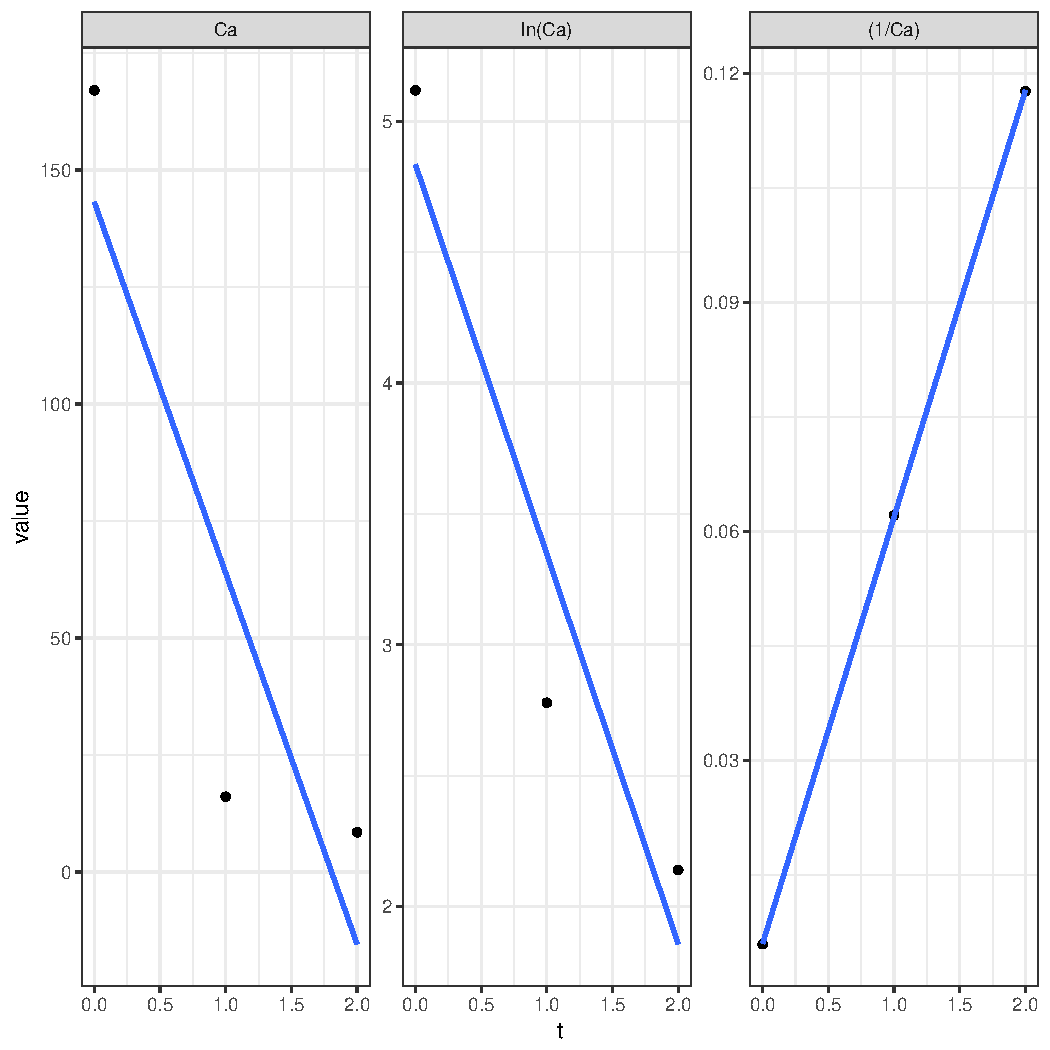
\includegraphics[width=\maxwidth]{figure/unnamed-chunk-4-1} 

\end{knitrout}

Linear model fit to (1/Ca) vs t since it has the best fit

\begin{knitrout}
\definecolor{shadecolor}{rgb}{0.969, 0.969, 0.969}\color{fgcolor}\begin{kframe}
\begin{alltt}
\hlstd{model} \hlkwb{<-} \hlstd{df} \hlopt
  \hlkwd{mutate}\hlstd{(}\hlkwc{Ca_inv} \hlstd{=} \hlnum{1}\hlopt{/}\hlstd{Ca)} \hlopt
  \hlkwd{lm}\hlstd{(Ca_inv} \hlopt{~} \hlstd{t,} \hlkwc{data} \hlstd{= .)}
\end{alltt}
\end{kframe}
\end{knitrout}

getting the model coefficients 
k = `r broom::tidy(model)$estimate[[1]]`

\begin{knitrout}
\definecolor{shadecolor}{rgb}{0.969, 0.969, 0.969}\color{fgcolor}\begin{kframe}
\begin{alltt}
\hlstd{broom}\hlopt{::}\hlkwd{tidy}\hlstd{(model)}
\end{alltt}
\begin{verbatim}
##          term    estimate    std.error statistic     p.value
## 1 (Intercept) 0.006086111 0.0002193283  27.74886 0.022932275
## 2           t 0.055829517 0.0001698910 328.61962 0.001937248
\end{verbatim}
\begin{alltt}
\hlstd{broom}\hlopt{::}\hlkwd{glance}\hlstd{(model)}
\end{alltt}
\begin{verbatim}
##   r.squared adj.r.squared        sigma statistic     p.value df   logLik
## 1 0.9999907     0.9999815 0.0002402622  107990.9 0.001937248  2 22.39244
##         AIC       BIC     deviance df.residual
## 1 -38.78488 -41.48905 5.772591e-08           1
\end{verbatim}
\end{kframe}
\end{knitrout}

\end{document}
